\section{ЭЛЕМЕНТЫ ТЕОРИИ ДВОЙСТВЕННОСТИ}

Для любой задачи линейного программирования можно сформулировать некоторую задачу, называемую двойственной. Решение каждой из этой пары задач часто  автоматически приводит к решению другой задачи, то есть количество решенных задач увеличивается вдвое. В некоторых случаях одна из  двойственных  задач проще и ее решать удобнее. Но важнее всего то, что во многих приложениях линейного программирования требуется решать обе двойственные задачи.  Поэтому изучение взаимосвязи этих задач очень полезно. Мы кратко опишем эту взаимосвязь, не останавливаясь подробно на обоснованиях.

\subsection{Симметрично-двойственные задачи}

Рассмотрим задачу линейного программирования в стандартной  форме.
\[
z = c_0 + c_1x_1 + \ldots + c_nx_n \rightarrow max;
\]
\[
\begin{cases}
a_{11}x_1 + a_{12}x_2 + \ldots + a_{1n}x_n \le b_1, \\
a_{21}x_1 + a_{22}x_2 + \ldots + a_{2n}x_n \le b_2, \\
\ldots\ldots\ldots\ldots\ldots\ldots\ldots\ldots\ldots\ldots\ldots \\
a_{m1}x_1 + a_{m2}x_2 + \ldots + a_{mn}x_n \le b_m;
\end{cases}
\]
\[ x_1, x_2, \ldots, x_n \ge 0. \]

Назовем эту задачу задачей 1. Построим по задаче 1 задачу 2, которая имеет следующий вид:
\[
f = c_0 + b_1y_1 + \ldots + b_my_m \rightarrow min;
\]
\[
\begin{cases}
a_{11}y_1 + a_{21}y_2 + \ldots + a_{m1}y_m \ge c_1, \\
a_{12}y_1 + a_{22}y_2 + \ldots + a_{m2}y_m \ge c_2, \\
\ldots\ldots\ldots\ldots\ldots\ldots\ldots\ldots\ldots\ldots\ldots \\
a_{1n}y_1 + a_{2n}y_2 + \ldots + a_{mn}y_m \ge c_n;
\end{cases}
\]
\[
y_1, y_2, \ldots, y_m \ge 0.
\]

Задача 2 построена по задаче 1 с помощью следующих правил:
\begin{enumerate}
\item Число переменных задачи 2 равно числу ограничений задачи 1.
\item Матрица системы ограничений задачи 2 является транспонированной по отношению к соответствующей матрице задачи 1, то есть, получена из нее заменой строк столбцами с сохранением порядка.
\item Свободный член целевой функции f задачи 2 равен свободному члену в  выражении целевой функции z задачи 1, а коэффициенты при переменных в выражении для f равны правым частям неравенств системы ограничений задачи 1.
\item Неравенства в системе ограничений задачи 2 имеют смысл <<$\geq{}$>>, а правые части этих неравенств равны коэффициентам при переменных  в целевой функции задачи 1.
\item Задача 2 является задачей на минимум, в то время как задача 1 является задачей на максимум.
\end{enumerate}

Отметим, что если рассматривать задачу 2 как исходную для построения двойственной задачи по сформулированным правилам, то двойственная задача будет равносильна задаче 1. Разумеется, при этом задачу 2 нужно сформулировать в стандартной форме.
\\\\
\primer{Исходная задача 1:
\[
z = 1 + 2x_1 - 3x_2 \rightarrow max;
\]
\[
y_1, y_2, y_3
\begin{cases}
2x_1 + 4x_2 \le 10, \\
4x_1 - 2x_2 \le 1, \\
5x_1 + 6x_2 \le 12;
\end{cases}
\]
\[
x_1, x_2 \ge 0.
\]

Двойственная задача 2:
\[
f = 1 + 10y_1 + y_2 + 12y_3 \rightarrow min;
\]
\[
\begin{cases}
2y_1 + 4y_2 + 5y_3 \ge 2, \\
4y_1 - 2y_2 + 6y_3 \ge -3;
\end{cases}
\]

Запишем задачу 2 в стандартной форме:
\[
f_1 = -1 - 10y_1 - y_2 - 12y_3 \rightarrow max;
\]
\[
\begin{cases}
-2y_1 - 4y_2 - 5y_3 \le -2, \\
-4y_1 + 2y_2 - 6y_3 \le 3;
\end{cases}
\]
\[
y_1, y_2, y_3 \le 0.
\]

Двойственная к ней задача:
\[
z_1 = -1 - 2x_1 + 3x_2 \rightarrow min;
\]
\[
\begin{cases}
-2x_1 - 4x_2 \ge -10, \\
-4x_1 + 2x_2 \ge -1, \\
-5x_1 - 6x_2 \ge -12;
\end{cases}
\]
\[
x_1, x_2 \ge 0.
\]
}

Полученная задача равносильна первоначально взятой задаче и совпадает с ней, если перейти к стандартной форме. Отмеченное свойство взаимности является причиной того, что пара задач (1;2) называется парой взаимно-двойственных задач.

\subsection{Экономический смысл взаимно-двойственных задач}

Рассмотрим \textit{задачу оптимального использования ресурсов} предприятием, которое производит n видов продукции:  $P_1, P_2, \ldots , P_n$ и использует для этого $m$ видов ресурсов $R_1, R_2, \ldots, R_m$. Будем считать, что ресурсы при необходимости можно продать, не изготавливая продукции. Если  $b_1, b_2 , \ldots, b_m$ --- наличные количества ресурсов;
$a_{ij}$ --- расход ресурса $R_i$ на изготовление единицы продукции $P_j$, а $x_j$ — плановое количество продукции $P_j$ , то переменные $x_1$, \ldots, $x_n$  должны удовлетворять системе неравенств:
\[
\begin{cases}
a_{11}x_1 + a_{12}x_2 + \ldots + a_{1n}x_n \le b_1, \\
a_{21}x_1 + a_{22}x_2 + \ldots + a_{2n}x_n \le b_2, \\
\ldots\ldots\ldots\ldots\ldots\ldots\ldots\ldots\ldots\ldots\ldots \\
a_{m1}x_1 + a_{m2}x_2 + \ldots + a_{mn}x_n \le b_m;
\end{cases}
\]
\[
x_1, x_2, \ldots, x_n \ge 0.
\]

Для максимизации прибыли от реализации продукции предприятие должно решить задачу на максимум для функции $z = c_1x_1 + \ldots + c_nx_n$, где  $c_1, c_2, \ldots, c_n$ — прибыли от реализации единицы соответствующего вида  продукции.

Пусть наше предприятие имеет возможность продать ресурсы некоторому другому предприятию или лицу.  Обозначим через
$y_1, \ldots, y_m$ соответствующие цены ресурсов $R_1, R_2, \ldots, R_m$.  Покупатель заинтересован в понижении цен, но продавец не будет продавать ресурсы, если продажа менее выгодна, чем  производство  продукции.  Станем на точку зрения покупателя и определим наиболее выгодные цены ресурсов с его точки зрения. При полной покупке ресурсов он должен минимизировать общую сумму выплаты за ресурсы:
\[
f = b_1y_1 + \ldots + b_my_m \rightarrow min.
\]

При этом стоимость ресурсов, идущих на изготовление единицы каждого вида продукции, не должна быть меньше, чем прибыль от ее реализации, иначе продавцу невыгодно продавать ресурсы. Поэтому цены $y_1, y_2, \ldots, y_m$ должны удовлетворять неравенствам:
\[
\begin{cases}
a_{11}y_1 + a_{21}y_2 + \ldots + a_{m1}y_m \ge c_1, \\
a_{12}y_1 + a_{22}y_2 + \ldots + a_{m2}y_m \ge c_2, \\
\ldots\ldots\ldots\ldots\ldots\ldots\ldots\ldots\ldots\ldots\ldots \\
a_{1n}y_1 + a_{2n}y_2 + \ldots + a_{mn}y_m \ge c_n;
\end{cases}
\]
\[
y_1, y_2, \ldots, y_m \ge 0.
\]

Таким образом, предприятие-покупатель ресурсов при назначении цен решает задачу линейного программирования двойственную по отношению к задаче, которую решает предприятие-производитель при составлении оптимального плана выпуска продукции. Величины $y^0_1, y^0_2, \ldots, y^0_m$, составляющие точку минимума для задачи покупателя, \textit{называют двойственными ценами (оценками) ресурсов}. Они имеют и более глубокий смысл, о котором речь пойдет ниже.

\subsection{Несимметрично-двойственные задачи}

Рассмотрим задачу линейного программирования в общем форме. Приведем эту задачу к стандартной форме с помощью рассмотренных выше приемов. Равенства в системе ограничений заменим парами противоположных  неравенств, а переменные,  принимающие значения  произвольного  знака, заменим разностями неотрицательных переменных. К полученной задаче в стандартной форме применим сформулированные выше правила построения двойственной задачи. Для простоты рассмотрим эту ситуацию на конкретном примере.

Исходная задача:
\[
z = 5 - x_1 + 3x_2 - x_3 \rightarrow min;
\]
\[
\begin{cases}
x_1 - 2x_2 + x_3 = 2, \\
x_1 + x_2 - x_3 \ge -3;
\end{cases}
\]
\[
x_1, x_2 \ge 0.
\]

Переменная  $x_3$ может принимать значения произвольного знака, поэтому полагаем $x_3 = x^{'}_3 - x^{''}_3$; $x^{'}_3, x^{''}_3 \ge 0$.   Запишем задачу в стандартной форме.
\[
z_1 = -5 + x_1 - 3x_2 + x^{'}_3 - x^{''}_3 \rightarrow max;
\]
\[
y_1, y_2, y_3
\begin{cases}
x_1 - 2x_2 + x^{'}_3 - x^{''}_3 \le 2, \\
-x_1 + 2x_2 - x^{'}_3 + x^{''}_3 \le -2, \\
-x_1 + x_2 - 3x^{'}_3 + 3x^{''}_3 \le 3;
\end{cases}
\]
\[
x_1, x_2, x^{'}_3, x^{''}_3 \ge 0.
\]

Построим двойственную задачу:
\[
f = -5 + 2y_1 - 2y_2 + 3y_3 \rightarrow min;
\]
\[
\begin{cases}
y_1 - y_2 - y_3 \ge 1, \\
-2y_1 + 2y_2 + y_3 \ge -3, \\
y_1 - y_2 - 3y_3 \ge 1, \\
-y_1 + y_2 + 3y_3 \ge -1;
\end{cases}
\]
\[
y_1, y_2, y_3 \ge 0.
\]

Отметим, что переменные $y_1$ и $y_2$ входят в эту задачу лишь в комбинации $y_1 - y_2$, а третье и четвертое неравенства системы ограничений двойственной задачи являются взаимно противоположными и могут быть заменены равенством $y_1 - y_2 - 3y_3 = 1$. Обозначая $y_1 - y_2$ через $y$, можем записать двойственную задачу в виде:
\[
f = -5 - 2y + 3y_3 \rightarrow min;
\]
\[
\begin{cases}
y - y_3 \ge 1, \\
-2y + y_3 \ge -3, \ \ y_3 \ge 0. \\
y - 3y_3 = 1;
\end{cases}
\]

Отметим, что эта же задача может быть получена из первоначальной задачи, записанной в виде задачи на максимум с неравенством типа <<<>> :
\[
z_1 = -5 + x_1 - 3x_2 + x_3 \rightarrow max;
\]
\[
y, y_3
\begin{cases}
x_1 - 2x_2 + x_3 = 2, \\
-x_1 + x_2 - 3x_3 \le 3;
\end{cases}
\]
\[
x_1, x_2 \ge 0,
\]
c помощью изложенного выше правила составления симметрично-двойственной задачи со следующими добавлениями:
\begin{enumerate}
\item[а)] если в исходной задаче в системе ограничений  есть  равенство, то в двойственной задаче соответствующая переменная не подчинена условию неотрицательности;
\item[б)] если в исходной задаче переменная не подчинена условию неотрицательности, то в двойственной задаче соответствующее ограничение  является равенством.
\end{enumerate}

В общем случае, если задачу общего вида сформулировать как задачу на максимум, все неравенства в системе ограничений которой имеют смысл <<$\leq{}$>>, то двойственную задачу можно сформулировать по правилам для симметрично двойственных задач с добавлениями
а) и б).

\subsection{Первая и вторая теоремы двойственности}

Все рассматриваемые ниже утверждения относятся к парам двойственных задач общего вида, то есть \textit{необязательно} симметрично-двойственных. \\

\teorema{Для всякой пары двойственных задач если исходная задача имеет решение, то двойственная задача также имеет решение, и оптимальные значения целевых функций этих задач совпадают, то есть $z_{max}=f_{min}$. Если исходная задача не имеет решения по причине  неограниченности целевой функции на области допустимых значений, то двойственная задача недопустима.} \\

Отметим, что первая теорема двойственности не позволяет по решению одной из задач найти точку оптимума другой. С ее помощью отыскивается лишь оптимальное значение целевой функции. Связь между точкой минимума и максимума пары двойственных задач определяет следующая:\\

\teorema{Для того, чтобы n-мерный вектор   удовлетворяющий системе ограничений исходной задачи, и m-мерный вектор $\{y^0_1, y^0_2, \ldots, y^0_m\}$  удовлетворяющий системе ограничений двойственной задачи, были соответственно точкой максимума исходной и точкой минимума  двойственной задач, необходимо и достаточно, чтобы выполнялись следующие условия:}
\[
\begin{cases}
y^0_1\left(a_{11}x^0_1 + a{12}x^0_2 + \ldots + a_{1n}x^0_n - b_1\right) = 0, \\
y^0_2\left(a_{21}x^0_1 + a_{22}x^0_2 + \ldots + a_{2n}x^0_n - b_2\right) = 0, \\
\ldots\ldots\ldots\ldots\ldots\ldots\ldots\ldots\ldots\ldots\ldots\ldots\ldots\ldots \\
y^0_m\left(a_{m1}x^0_1 + a_{m2}x^0_2 + \ldots + a_{mn}x^0_n - b_m\right) = 0, \\
x^0_1\left(a_{11}y^0_1 + a_{21}y^0_2 + \ldots + a_{m1}y^0_m - c_1\right) = 0, \\
x^0_2\left(a_{12}y^0_1 + a_{22}y^0_2 + \ldots + a_{m2}y^m_0 - c_2\right) = 0, \\
\ldots\ldots\ldots\ldots\ldots\ldots\ldots\ldots\ldots\ldots\ldots\ldots\ldots\ldots \\
x^0_n\left(a_{1n}y^0_1 + a_{2n}y^0_2 + \ldots + a_{mn}y^0_m - c_n\right) = 0.
\end{cases}
\]

Вторая теорема двойственности содержит равенства, которые называются условиями дополнительной нежесткости. Она позволяет решать следующие задачи:
\begin{enumerate}
\item[1)] определять оптимальный план одной из двойственных задач, если известно решение другой;
\item[2)] проверять, не решая задачи, является ли некоторая совокупность чисел оптимальным планом одной из двойственных задач.
\end{enumerate}

\primer{
Пусть дана задача:
\[
z = x_1 + x_2 + x_3 \rightarrow max;
\]
\[
y_1, y_2
\begin{cases}
2x_1 + 3x_2 - x_3 \le 2, \\
x_1 - x_2 + 2x_3 \le 3;
\end{cases}
\]
\[
x_1, x_2, x_3 \ge 0.
\]

Двойственную задачу
\[
f = 2y_1 + 3y_2 \rightarrow min;
\]
\[
\begin{cases}
2y_1 + y_2 \ge 1, \\
3y_1 - y_2 \ge 1, \\
-y_1 + 2y_2 \ge 1;
\end{cases}
\]
\[
y_1, y_2 \ge 0.
\]
можно решить графически (рис.3.1.).

\begin{figure}[h!]
\center{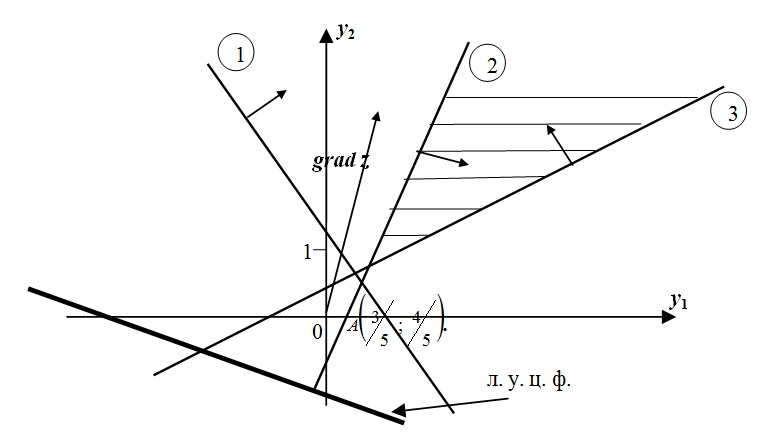
\includegraphics[width=1\linewidth]{pictures/picturefile_3_1}}
\caption*{Рис. 3.1. Графическое решение двойственной задачи}
\label{picture_3_1}
\end{figure}

Точкой минимума двойственной задачи является точка $A\left(\frac{3}{5};\frac{4}{5}\right)$. $z_{max} = f_{min} = f(A) = 2 \cdot \frac{3}{5} + 3 \cdot \frac{4}{5} = \frac{6}{6} + \frac{12}{5} = \frac{18}{5}$. Для определения  точки максимума исходной задачи составим условия дополнительной нежесткости:
\[
\begin{cases}
y^0_1\left(2x^0_1 + 3x^0_2 - x^0_3 - 2\right) = 0, \\
y^0_1\left(x^0_1 - x^0_2 + 2x^0_n - 3\right) = 0, \\
x^0_1\left(2y^0_1 + y^0_1 - 1\right) = 0, \\
x^0_2\left(3y^0_1 - y^0_2 - 1\right) = 0, \\
x^0_3\left(-y^0_1 + 2y^0_2 - 1\right) = 0.
\end{cases}
\]

Подставим в эти равенства $y^0_1 = \frac{3}{5}; y^0_2 = \frac{4}{5}$ Учитывая, что четвертое и пятое равенства при этом выполняются при всех $x^0_3$ и $x^0_2$ , для определения $x^0_1, x^0_2, x^0_3$ получаем систему уравнений
\[
\begin{cases}
2x^0_1 + 3x^0_2 - x^0_3 = 3, \\
x^0_1 - x^0_2 + 2x^0_3 = 3, \\
x^0_1 = 0,
\end{cases}
\]
которая равносильна системе
\[
\begin{cases}
3x^0_2 - x^0_3 = 2, \\
-x^0_2 + 2x^0_3 = 3, \\
x^0_1 = 0,
\end{cases}
\]

Ее решение: $x^0_1 = 0; x^0_2 = \frac{7}{5}; x^0_3 = \frac{11}{5}$. Таким образом, точка максимума исходной задачи $\left(0; \frac{7}{5}; \frac{11}{5}\right)$.
} \\

\primer{
Будет ли план $\overrightarrow{x}$ = \{1; 1: 1\}  оптимальным планом задачи
\[
z = x_1 + 2x_2 + 3x_3 \rightarrow max;
\]
\[
y_1, y_2
\begin{cases}
x_1 - x_2 - x_3 \le 1, \\
x_1 + x_2 - x_3 \le 1;
\end{cases}
\]
\[
x_1, x_2, x_3 \ge 0?
\]

Составим двойственную задачу:
\[
f = y_1 + y_2 \rightarrow min;
\]
\[
\begin{cases}
y_1 + y_2 \ge 1, \\
-y_1 + y_2 \ge 2, \\
-y_1 - y_2 \ge 3;
\end{cases}
\]
\[
y_1, y_2 \ge 0.
\]

Составим условия дополнительной нежесткости:
\[
\begin{cases}
y^0_1\left(x^0_1 - x^0_2 - x^0_3 - 1\right) = 0, \\
y^0_2\left(x^0_1 + x^0_2 - x^0_n - 1\right) = 0, \\
x^0_1\left(y^0_1 + y^0_2 - 1\right) = 0, \\
x^0_2\left(-y^0_1 + y^0_2 - 2\right) = 0, \\
x^0_3\left(-y^0_1 - y^0_2 - 3\right) = 0.
\end{cases}
\]

Подставим в эти равенства $x^0_1 = x^0_2 = x^0_3 = 1$.

Получим систему уравнений
\[
\begin{cases}
-2y^0_1 = 0, \\
y^0_1 + y^0_2 = 1, \\
-y^0_1 + y^0_2 = 2, \\
-y^0_1 - y^0_2 = 3,
\end{cases}
\]
которая является несовместной. Следовательно, рассматриваемый план оптимальным планом не будет.
}

\subsection{ Третья теорема двойственности}

Пусть некоторая задача линейного программирования решена и получено некоторое значение $z_{max}$. При изменении правых частей ограничений $b_1, b_2, \ldots, b_m$  задача меняется и, в конечном счёте, меняется значение $z_{max}$. Будем рассматривать zmax   как функцию величин $b_1, b_2, \ldots, b_m$, то есть рассмотрим функцию $z_{max}(b_1, b_2, \ldots, b_m)$. \\

\teorema{В оптимальном плане двойственной задачи координата $y^0_1$ численно равна частной производной функции $z_{max}(b_1, b_2, \ldots, b_m)$ по переменной $b_i$, то есть
\[
\frac{\partial{z_{max}}}{\partial{b_i}} = y^0_1; \ \ i = 1, 2, \ldots, m.
\]}

Эта теорема может быть истолкована и следующим образом. Пусть величинам $b_1, b_2, \ldots, b_m$  придаются приращения $\Delta b_1, \Delta b_2, \ldots, \Delta b_m$. Функция $z_{max}(b_1, b_2, \ldots, b_m)$ получает приращение $\Delta z_{max}$. По сформулированной теореме при малых приращениях $\Delta b_1, \Delta b_2, \ldots, \Delta b_m$ справедливо следующее приближенное равенство
\[
\Delta z_{max} \approx y^0_1 \Delta b_1 + y^0_2 \Delta b_2 + \ldots + y^0_m \Delta b_m.
\eqno(3.1)
\]

На самом деле функция $z_{max}(b_1, b_2, \ldots, b_m)$ такова, что при изменении $\Delta b_i$ в некоторых пределах, равенство (3.1) является точным. При этом величины $\Delta b_i$ могут быть и не малыми по сравнению с $b_i$.

Определить эти пределы изменения величин $\Delta b_i$ можно с помощью второй теоремы двойственности. Равенство (3.1) будет точным, если при изменении $b_i$ величины $y^0_i$ не изменяются.  Пределы же изменения приращений $\Delta b_i$, при которых оптимальный план двойственной задачи не меняется, можно определить следующим образом. Придадим фиксированным значениям $b^0_1, b^0_2, \ldots, b^0_m$ неопределенные приращения $\Delta b_1, \Delta b_2, \ldots, \Delta b_m$ и рассмотрим условия дополнительной нежесткости с наращенными значениями $b_i = b^0_i + \Delta b_i$, в которые подставим старые значения $y^0_i$. Относительно оптимального плана исходной задачи $x^0_1, x^0_2, \ldots, x^0_n$ получится система линейных уравнений, которую можно решить при определенных условиях с помощью, например,  метода  обратной матрицы. Получим зависимость
\[
x^0_i = x^0_i\left(\Delta b_1, \Delta b_2, \ldots, \Delta b_m\right)
\]
оптимального плана от приращений. Поскольку $x^0_i$ должны удовлетворять неравенствам $x^0_i \ge 0, i = 1, 2, \ldots, n$, а также системе ограничений исходной задачи, то мы получим систему условий,  которым должны удовлетворять $\Delta b_i$, чтобы оптимальный план двойственной задачи не менялся. Эта область изменения $\Delta b_i$ называется областью устойчивости двойственных оценок. \\

\primer{Рассмотрим пару двойственных задач примера 3.2. Оптимальный план двойственной задачи здесь $y^0_1 = \frac{3}{5}; y^0_2 = \frac{4}{5}$. Наращенные значения правых частей ограничений исходной задачи равны: $b_1 = 2 + \Delta b_1, b_2 = 3 + \Delta b_2$. Условия дополнительной нежесткости имеют вид
\[
\begin{cases}
\frac{3}{5}\left(2x^0_1 + 3x^0_2 - x^0_3 - 2 - \Delta b_1\right) = 0, \\
\frac{4}{5}\left(x^0_1 - x^0_2 + 2x^0_3 - 3 - \Delta b_2\right) = 0, \\
x^0_1\left(2 \cdot \frac{3}{5} + \frac{4}{5} - 1\right) = 0, \\
x^0_2\left(\frac{9}{5} - \frac{4}{5} - 1\right) = 0, \\
x^0_3\left(-\frac{3}{5} + \frac{8}{5} - 1\right) = 0.
\end{cases}
\]

Четвёртое и пятое равенства — тождества, а из третьего следует, что $x^0_1 = 0$. Для $x^0_2$ и $x^0_3$ получаем систему равенств
\[
\begin{cases}
3x^0_2 - x^0_3 = 2 + \Delta b_1, \\
-x^0_2 + 2x^0_3 3 + \Delta b_2.
\end{cases}
\]

Отсюда
\[
x^0_2 = \frac{2}{5}\left(2 + \Delta b_1\right) + \frac{1}{5}\left(3 + \Delta b_2\right) = \frac{7}{5} + \frac{2}{5} \Delta b_1 + \frac{1}{5} \Delta b_2,
\]
\[
x^0_3 = \frac{1}{5}\left(2 + \Delta b_1\right) + \frac{3}{5}\left(3 + \Delta b_2\right) = \frac{11}{5} + \frac{1}{5} \Delta b_1 + \frac{3}{5} \Delta b_2.
\]

\begin{figure}[h!]
\center{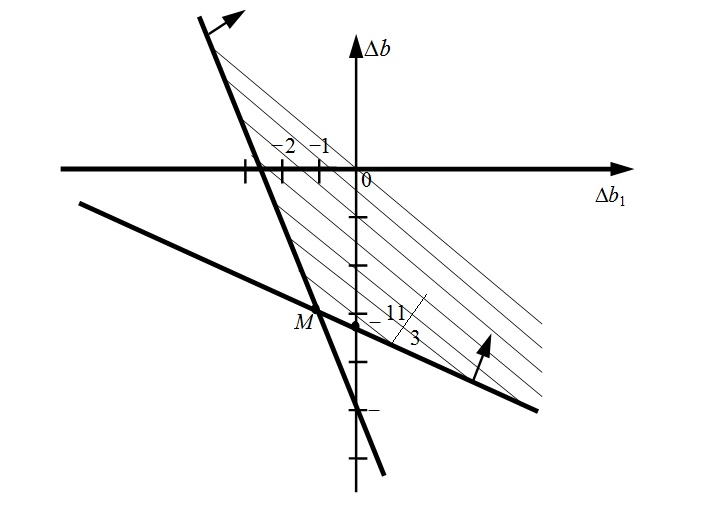
\includegraphics[width=1\linewidth]{pictures/picturefile_3_2}}
\caption*{Рис. 3.2. Область устойчивости двойственных оценок примера 3.4}
\label{picture_3_2}
\end{figure}

Приращения $\Delta b_1$ и $\Delta b_2$ должны удовлетворять неравенствам
\[
\begin{cases}
\frac{7}{5} + \frac{2}{5} \Delta b_1 + \frac{1}{5} \Delta b_2 \ge 0, \\
\frac{11}{5} + \frac{1}{5} \Delta b_1 + \frac{3}{5} \Delta b_2 \ge 0.
\end{cases}
\]

Система ограничений исходной задачи с правыми частями $2 + \Delta b_1$ и $3 + \Delta b_2$ удовлетворяется автоматически. Таким образом,  можно изобразить на плоскости  область  изменения величин $\Delta b_1, \Delta b_2$,  в которой оптимальный план двойственной задачи не меняется.

В области, изображенной на рис. 3.2, приращение $\Delta z_{max}$ может быть найдено по точной формуле:
\[
\Delta z_{max} = y^0_1 \Delta b_1 + y^0_2 \Delta b_2 = \frac{3}{5} \Delta b_1 + \frac{4}{5} \Delta b_2.
\]
}

\subsection{Послеоптимизационный анализ}

Пусть рассматривается задача оптимального использования ресурсов. Пусть решена и сама эта задача, и двойственная к ней. Знание двойственных оценок $y^0_1, y^0_2, \ldots, y^0_m$ позволяет судить о том, насколько ценным в производстве является данный ресурс. Если величина $y^0_i \neq 0$ то в силу условий дополнительной нежесткости ресурс при реализации оптимального плана выпуска продукции используется полностью. Не полностью используются ресурсы, для которых $y^0_i = 0$. Таким образом, двойственные оценки ресурсов характеризуют их дефицитность. Различные варианты наращивания ресурсов (или их сокращения) приводят к разным величинам изменения оптимальной прибыли $\Delta z_{max}$. Чем больше величина $y^0_i$, тем больше приращение оптимальной прибыли мы получим при увеличении объема ресурса $R_i$ на 1 единицу. В этом и заключается более глубокий смысл двойственных оценок ресурсов по сравнению с изложенным ранее.

При анализе возможностей  расширения производства знание двойственных оценок ресурсов играет большую роль. Обычно такой анализ называют послеоптимизационным, поскольку он выполняется после  решения прямой и двойственной задач. Здесь, однако, следует помнить, что для использования двойственных оценок в экономическом анализе нужно знать область их устойчивости, то есть область изменения ресурсов, в которой двойственные оценки ресурсов не меняются.

\subsection{Двойственный симплекс-метод для пары\\
симметрично-двойственных задач}

Если размерности исходной и двойственной задач велики, то определение решения одной из задач по решению другой с помощью условий дополнительной нежесткости затруднительно. В этом случае применяют двойственный симплекс-метод, который позволяет по последней симплекс-таблице одной из задач прочесть решение двойственной задачи. Этот метод мы рассмотрим сначала в упрощенной форме для пары симметрично-двойственных задач, причем для такой пары, в которой одна из задач после уравнивания неравенств системы ограничений имеет эту систему ограничений в допустимом базисном виде, то есть, может решаться симплекс-методом непосредственно. В следующем параграфе будет рассмотрен подобный метод для произвольной задачи в канонической форме.

Пусть при уравнивании системы ограничений исходной задачи мы ввели переменные $x_{n + 1}, x_{n + 2}, \ldots, x_{n + m}$. Эти переменные играют роль базисных. При уравнивании системы ограничений двойственной задачи вводятся переменные $y_{m + 1}, y_{m + 2}, \ldots, y_{m + n}$, которые также играют роль базисных.  Определим соответствие между переменными исходной и двойственной задач, сопоставляя каждой свободной переменной исходной задачи базисную переменную двойственной в соответствии с порядком следования номеров, а каждой базисной переменной исходной задачи --- свободную переменную двойственной задачи. Запишем это соответствие в таком виде:
\[
\begin{array}{cccccccc}
x_1, & x_2, & \ldots, & x_n, & x_{n + 1}, & x_{n + 2}, & \ldots, & x_{n + m} \\
\updownarrow &\updownarrow &\updownarrow  &\updownarrow  &\updownarrow  &\updownarrow  &\updownarrow  &\updownarrow  \\
y_{m + 1}, & y_{m + 2}, & \ldots, & y_{m + n}, & y_1, & y_2, & \ldots, & y_m.
\end{array}
\eqno(F)
\]

Отметим, что это соответствие переменных устанавливает взаимосвязь базисных решений данной и двойственной задач. Если составлена таблица, аналогичная симплекс-таблице, по базисному решению данной задачи, то соответствующее базисное решение двойственной задачи прочитывается по последней строке этой симплекс-таблицы с использованием построенного выше соответствия переменных. А именно, значение $y_i$ в базисном решении двойственной задачи прочитывается в строке целевой функции симплекс-таблицы в столбце переменной $x_j$, соответствующей переменной $y_i$, по соответствию переменных $(F)$. Эта взаимосвязь базисных решений сохраняется при всевозможных преобразованиях замещения данной таблицы в предположении, что в двойственной задаче происходит переход к соответствующему новому базисному решению.

Пусть одна из задач решена симплекс-методом и получена последняя симплекс-таблица. Решение (точка оптимума) другой задачи может быть прочитано по последней симплекс-таблице с использованием соответствия переменных $(F)$. \\

\primer{
 Рассматривается пара двойственных задач:
\[
1) z = -x_1 + x_2 \rightarrow max; \ \ \ \ \ \ \ \ \ \ \ \ \ \ \ \ \ \ \ 2) f = y_1 + 2y_2 + 3y_3 \rightarrow min;
\]
\[
\begin{cases}
x_1 - 2x_2 \le 1, \\
-2x_1 + x_2 \le 2, \\
3x_1 + x_2 \le 3;
\end{cases} \ \ \ \ \ \ \ \ \ \ \ \ \ \ \ \ \ \ \ \ \ \ \ \ \ \ \ \ \
\begin{cases}
y_1 - 2y_2 + 3y_3 \ge -1, \\
-2y_1 + y_2 + y_3 \ge 1;
\end{cases}
\]
\[
x_1 \ge 0, x_2 \ge 0. \ \ \ \ \ \ \ \ \ \ \ \ \ \ \ \ \ \ \ \ \ \ \ \ \ \ \ \ \ \ \ \ y_1 \ge 0, y_2 \ge 0, y_3 \ge 0.
\]

После уравнивания неравенств задачи имеют следующий вид:
\[
1) z = -x_1 + x_2 \rightarrow max; \ \ \ \ \ \ \ \ \ \ \ \ \ \ \ \ \ \ \ 2) f = y_1 + 2y_2 + 3y_3 \rightarrow min;
\]
\[
\begin{cases}
x_1 - 2x_2 + x_3 = 1, \\
-2x_1 + x_2 + x_4 = 2, \\
3x_1 + x_2 + x_5;
\end{cases} \ \ \ \ \ \ \ \ \ \ \ \ \ \ \ \ \ \
\begin{cases}
y_1 - 2y_2 + 3y_3 - y_4 = -1, \\
-2y_1 + y_2 + y_3 - y_5 = 1;
\end{cases}
\]
$\ \ \ \ \ \ \ \ \ \ x_1, x_2, \ldots, x_5 \ge 0. \ \ \ \ \ \ \ \ \ \ \ \ \ \ \ \ \ \ \ \ \ \ \ \ \ \ \ y_1, y_2, \ldots, y_5 \ge 0.$ \\

Составим соответствие переменных:
\[
\begin{array}{ccccc}
x_1, & x_2, & x_3, & x_4, & x_5 \\
\updownarrow &\updownarrow &\updownarrow  &\updownarrow  &\updownarrow  \\
y_1, & y_2, & y_3, & y_4, & y_5.
\end{array}
\]

Решая исходную задачу симплекс-методом, получаем следующую последнюю симплекс-таблицу: \\

\begin{tabular}{| c | c | c | c | c | c | c |}
\hline
Базисные переменные & Свободные члены & $x_1$ & $x_2$ & $x_3$ & $x_4$ & $x_5$ \\ \hline
$x_3$ & 28/5 & 0 & 0 & 1 & 7/5 & 3/5 \\ \hline
$x_2$ & 12/5 & 0 & 1 & 0 & 3/5 & 2/5 \\ \hline
$x_1$ & 1/5 & 0 & 0 & 0 & 4/5 & 1/5 \\ \hline
$z$ & 11/5 & 0 & 0 & 0 & 4/5 & 1/5 \\ \hline
\end{tabular} \\ \\

По первой теореме двойственности и в соответствии со сказанным выше $f_{min} = \frac{11}{5}$; точка максимума имеет координаты
\[
y^0_1 = 0; y^0_2 = \frac{4}{5}; y^0_3 = \frac{1}{5}.
\]
}

Двойственный симплекс-метод можно распространить и на произвольные задачи, однако, при этом он заметно усложняется.

\subsection{ Метод последовательного уточнения оценок. Обобщенный двойственный симплекс-метод}

Метод последовательного уточнения оценок применяется к задаче линейного программирования в канонической форме
\[
z = c_0 + \left(\overrightarrow{c}, \overrightarrow{x}\right) \rightarrow max,
\]
\[
A\overrightarrow{x} = \overrightarrow{b}, \overrightarrow{x} \ge \overrightarrow{0},
\]
где A --- ($m \times n$) — матрица. Он так же, как и симплекс метод заключается в таком последовательном переходе от одного n-мерного вектора $\overrightarrow{x}$ к другому, при котором после конечного числа переходов либо получается оптимальное решение задачи, либо устанавливается ее неразрешимость. Однако в отличие от симплекс-метода эти последовательно получаемые векторы, вообще говоря, не являются допустимыми решениями системы ограничений (допустимыми планами), а являются в некотором смысле <<почти>> допустимыми, так называемыми \textit{псевдопланами} данной задачи. Эти псевдопланы являются базисными решениями системы уравнений задачи, но не обязательно удовлетворяют условиям неотрицательности. Процесс перехода от одного псевдоплана к другому построен так, что как только очередной псевдоплан $\overrightarrow{x}$ оказывается неотрицательным, т.е. допустимым планом задачи, он является одновременно и оптимальным решением этой задачи. Каждому псевдоплану по его определению соответствует опорное решение системы ограничений двойственной задачи. При этом каждому следующему певдоплану соответствует лучшее, чем предыдущее, опорное решение двойственной задачи. Оптимальному решению данной задачи соответствует оптимальное решение двойственной. Таким образом, метод последовательного уточнения оценок — это применение обычного симплекс метода к двойственной задаче, дополненное на каждой итерации построением n-мерного вектора $\overrightarrow{x}$, являющегося псевдопланом данной задачи. Геометрически этот метод можно истолковать как построение последовательности псевдопланов $\overrightarrow{x_1}, \overrightarrow{x_2}, \ldots, \overrightarrow{x_5}$, являющихся точками n-мерного пространства $R^n$. находящимися вне допустимого многогранника. При этом каждый следующий вектор этой последовательности определяет гиперплоскость уровня целевой функции, которая находится ближе к области допустимых значений, чем предыдущая. Через конечное число шагов мы получим точку  $\overrightarrow{x_5}$, принадлежащую допустимому многограннику, либо выяснится, что допустимый многогранник пуст. Перейдем к более детальному описанию метода. Предположим, что система ограничений задачи в канонической форме приведена к базисному виду, который, вообще говоря, не является допустимым и пусть из целевой функции исключены базисные переменные. Составим таблицу, аналогичную симплекс таблице. Отличие заключается лишь в том, что эта таблица составляется по, вообще говоря, недопустимому базисному виду системы уравнений. Эту таблицу будем называть обобщенной симплекс таблицей. Коэффициенты $\Delta_j$ при свободных переменных в последней строке этой таблицы назовем оценками свободных переменных для данного базисного решения. \\


\opredelenie{Базисное решение системы ограничений задачи линейного программирования в канонической форме называется псеввдопланом этой задачи, если для него все оценки свободных переменных неотрицательны ($\Delta_j \ge 0$).} \\

\statement{Если псевдоплан задачи линейного программирования в канонической форме является допустимым планом этой задачи, то он одновременно является оптимальным планом.} \\

\so{Доказательсво}. Если псевдоплан является допустимым, то составленная нами таблица будет обычной симплекс таблицей, у которой все коэффициенты $\Delta_j = -\gamma_j$ в последней строке неотрицательны. Значит, получена последняя симплекс таблица и соответствующий план будет оптимальным, что и требовалось доказать. \\

\statement{Если псевдоплан задачи линейного программирования в канонической форме имеет отрицательную компоненту $b_k < 0$, а все коэффициенты k-ой строки таблицы неотрицательны $a_{kj} \ge 0$, то задача не  имеет решения по причине отсутствия допустимых решений системы ограничений.} \\

\so{Доказательство}. $k$-ая строка таблицы отвечает уравнению
\[
x_k = b_k - \sum_{j} a_{kj}x_j,
\]
которое при наших условиях не может иметь неотрицательного решения. Следовательно, система ограничений задачи допустимых решений не имеет. Утверждение доказано.

Рассмотрим некоторую процедуру перехода от одной обобщенной симплекс таблицы к другой, которая соответствует переходу от одного псевдоплана к другому. Если таблица соответствует псевдоплану, который не является допустимым планом задачи, то в столбце свободных членов среди отрицательных элементов выберем максимальное по модулю отрицательное число $b_k < 0$ и в $k$-ой строке отметим все отрицательные числа $a_{kj} < 0$. Если таковых не окажется, то в силу утверждения 2 задача является недопустимой и решения не имеет. Среди отмеченных элементов k-ой строки выберем элемент $a_{kj_0}$, на котором достигается  $\underset{j}{min}\left(-\frac{\Delta_j}{a_{kj}}\right)$. Если таких элементов несколько, то выбираем любой из них. Этот выбранный элемент берем в качестве разрешающего и производим операцию замещения в нашей таблице, выводя переменную $x_k$ из числа базисных и вводя в число базисных переменную $x_{j_0}$. Отметим, что новая таблица тоже будет отвечать псевдоплану задачи вследствие правила выбора разрешающего элемента. При этом в новой таблице значение целевой функции $\gamma_0$ будет меньше, чем в старой. Таким образом, справедливо \\

\statement{При описанном переходе от обобщенной симплекс таблицы, отвечающей некоторому псевдоплану, либо выяснится, что исходная задача не имеет решения, либо получится новая таблица, отвечающая некоторому новому псевдоплану. При этом значение целевой функции на новом псевдоплане будет меньше, чем на старом.} \\

Описанные итерации повторяются до тех пор, пока очередной псевдоплан не станет допустимым планом задачи, который одновременно будет оптимальным планом. Важно заметить, что каждому псевдоплну однозначно сопоставляется некоторый опорный план двойственной задачи. Действительно, если система ограничений приведена к базисному виду, а из целевой функции исключены базисные переменные, то базисные переменные можно убрать, превращая уравнения в неравенства. Для полученной формы задачи построим двойственную задачу. Приведение данной и двойственной задач к каноническому виду дает пару задач с одинаковым числом переменных, которые можно привести во взаимно однозначное соответствие вида $(F)$. С использованием этого соответствия и обобщенной симплекс таблицы мы можем, как и в предыдущем параграфе каждому псевдоплану сопоставить допустимый план двойственной задачи. Наши итерации, по сути, являются переходами от одного опорного решения двойственной задачи к другому с улучшением значения целевой функции.  Поскольку координаты опорного решения двойственной задачи совпадают с оценками свободных переменных псевдоплана, то мы, по сути, последовательно улучшаем эти оценки. Отсюда происходит название рассмотренного метода. \\

\statement{Если исходная задача не имеет решения по причине неограниченности целевой функции на области допустимых значений, то она не имеет ни одного псевдоплана.} \\

\so{Доказательство}. Предположим противное, т. е. что существует хотя бы один псевдоплан. Ему должен соответствовать допустимый план двойственной задачи. Но по первой теореме двойственности при наших условиях двойственная задача должна быть недопустимой, т. е. ее область допустимых значений пуста. Пришли к противоречию. Утверждение 4 доказано.

\primer{
 Решить задачу
\[
z = 16 - x_1 - x_2 \rightarrow max;
\]
\[
\begin{cases}
x_1 + x_2 \le 8, \\
x_1 - x_2 \ge 4, \\
x_1 + 2x_2 \ge 6;
\end{cases}
\]
\[
x_1, x_2 \ge 0.
\]

Построим двойственную задачу
\[
f = 16 + 8y_1 - 4y_2 - 6y_3 \rightarrow min;
\]
\[
\begin{cases}
y_1 - y_2 - y_3 \ge -1, \\
y_1 + y_2 - 2y_3 \ge -1;
\end{cases}
\]
\[
y_1, y_2, y_3 \ge 0.
\]

Приведем исходную и двойственную задачи к каноническому виду.
\[
z = 16 - x_1 - x_2 \rightarrow max; \ \ \ \ \ \ \ \ \ \  f = 16 + 8y_1 - 4y_2 - 6y_3 \rightarrow min;
\]
\[
\begin{cases}
x_1 + x_2 + x_3 = 8, \\
-x_1 + x_2 + x_4 = -4, \\
-x_1 - 2x_2 + x_5 = -6;
\end{cases} \ \ \ \ \ \ \ \ \ \
\begin{cases}
-y_1 + y_2 + y_3 + y_4 = 1, \\
-y_1 - y_2 + 2y_3 + y_5 = 1;
\end{cases}
\]
$\ \ \ \ \ \ \ \ \ \ \ \ \ x_1, x_2, x_3, x_5 \ge 0.\ \ \ \ \ \ \ \ \ \ \ \ \ \ \ \ \ \ \ \ \ \ \  y_1, y_2 , y_3 \ge 0.$ \\

Составим обобщенную симплекс таблицу исходной задачи.

\begin{table}[h!]
\caption*{\hspace{0.8\linewidth} \textit{Таблица 1}}
\begin{center}
\begin{tabular}{|c|c|c|c|c|c|c|}
\hline
\begin{tabular}[c]{@{}c@{}}Базисные \\ переменные\end{tabular} & \begin{tabular}[c]{@{}c@{}}Свободные\\ члены\end{tabular} & $x_1$ & $\downarrow x_2$ & $x_3$ & $x_4$ & $x_5$ \\ \hline
$x_3$                                                           & 8                                                         & 1    & 1                              & 1    & 0    & 0    \\ \hline
$x_4$                                                           & -4                                                        & -1   & 1                              & 0    & 1    & 0    \\ \hline
\cellcolor[gray]{0.75} $\leftarrow x_5$                         &\cellcolor[gray]{0.75} -6            &\cellcolor[gray]{0.75} -1   &\cellcolor[gray]{0.75} [-2]       &\cellcolor[gray]{0.75} 0    &\cellcolor[gray]{0.75} 0    &\cellcolor[gray]{0.75} 1    \\ \hline
$z$                                                              & 16                                                        & 1    & 1                              & 0    & 0    & 0    \\ \hline
\end{tabular}
\end{center}
\end{table}

Таблица отвечает псевдоплану. Согласно соответствию переменных (F) этому псевдоплану соответствует допустимый план  (0, 0, 0, 1, 1) двойственной задачи. По сформулированному выше правилу выбираем разрешающий элемент (-2) и перейдем к следующей таблице.

\begin{table}[h!]
\caption*{\hspace{0.8\linewidth} \textit{Таблица 2}}
\begin{center}
\begin{tabular}{|c|c|c|c|c|c|c|}
\hline
\begin{tabular}[c]{@{}c@{}}Базисные \\ переменные\end{tabular} & \begin{tabular}[c]{@{}c@{}}Свободные\\ члены\end{tabular} & $\downarrow x_1$ & $x_2$ & $x_3$ & $x_4$ & $x_5$ \\ \hline
$x_3$                                                          & 5                                                         & 1/2              & 0     & 1     & 0     & 1/2   \\ \hline
\cellcolor[gray]{0.75} $\leftarrow x_4$  &\cellcolor[gray]{0.75} -7  &\cellcolor[gray]{0.75} [-3/2]  &\cellcolor[gray]{0.75} 0 &\cellcolor[gray]{0.75} 0     &\cellcolor[gray]{0.75} 1     &\cellcolor[gray]{0.75} 1/2   \\ \hline
$x_5$                                                          & 3                                                         & 1/2              & 1     & 0     & 0     & -1/2  \\ \hline
$z$                                                            & 13                                                        & 1/2              & 0     & 0     & 0     & 1/2   \\ \hline
\end{tabular}
\end{center}
\end{table}

Эта таблица тоже соответствует псевдоплану, а также допустимому плану (0, 0, $\frac{1}{2}$, $\frac{1}{2}$, 0) двойственной задачи.

\begin{table}[h!]
\caption*{\hspace{0.8\linewidth} \textit{Таблица 3}}
\begin{center}
\begin{tabular}{|c|c|c|c|c|c|c|}
\hline
\begin{tabular}[c]{@{}c@{}}Базисные \\ переменные\end{tabular} & \begin{tabular}[c]{@{}c@{}}Свободные\\ члены\end{tabular} & $x_1$ & $x_2$ & $x_3$ & $x_4$ & $x_5$ \\ \hline
$x_3$                                                          & 8/3                                                       & 0     & 0     & 1     & 1/3   & 2/3   \\ \hline
$x_1$                                                          & 14/3                                                      & 1     & 0     & 0     & -2/3  & -1/3  \\ \hline
$x_2$                                                          & 2/3                                                       & 0     & 1     & 0     & 1/3   & -1/3  \\ \hline
$z$                                                            & 32/3                                                      & 0     & 0     & 0     & 1/3   & 2/3   \\ \hline
\end{tabular}
\end{center}
\end{table}

В последней симплекс таблице псевдоплан является допустимым планом, а, следовательно, оптимальным планом задачи. Получаем ответ в исходной задаче: $z_{max} = \frac{32}{3}; точка максимума (\frac{14}{3}; \frac{2}{3})$. Решение двойственной задачи тоже прочитывается по последней симплекс таблице: $f_{min} = \frac{32}{3}$; точка минимума (0; $\frac{1}{3}$; $\frac{2}{3}$).
}

Отметим, что для получения решения исходной задачи методом последовательного уточнения оценок строить двойственную задачу, как в рассмотренном примере, совсем не обязательно. Рассмотренный пример показывает, по сути, равносильность нашего метода и двойственного симплекс метода, рассмотренного в предыдущем параграфе. Поэтому в дальнейшем метод последовательного уточнения оценок мы часто будем называть тоже \textit{двойственным симплекс методом}. Этот метод удобен в случае, когда удалось выйти на псевдоплан. Такая ситуация встречается довольно часто (см., например, примеры 5.3 и 5.4). В общем же его применение может привести к сокращению количества итераций, необходимых в среднем для решения произвольной задачи линейного программирования в канонической форме по сравнению с применением простого симплекс метода или его модификаций типа метода искусственного базиса. Следующий составной алгоритм часто называют \textit{обобщенным двойственным симплекс методом}.
\begin{enumerate}
\item[1.] Привести систему ограничений задачи к базисному виду и исключить базисные переменные из целевой функции.
\item[2.] Проверить, будет ли полученное базисное решение допустимым планом задачи. Если да, то решить задачу обычным симплекс методом и перейти к п. 5, иначе перейти к п. 3.
\item[3.] Проверить, будет ли полученное базисное решение псевдопланом задачи. Если да, то решить задачу двойственным симплекс методом и перейти к п. 5, иначе перейти к п. 4.
\item[4.] Перейти к следующему базисному виду системы ограничений и перейти к п. 2.
\item[5.] Конец.
\end{enumerate}

\subsection{Понятие об устойчивости задач линейного программирования. Регуляризация неустойчивых задач}

Содержание этого параграфы важно для практического применения линейного программирования и существенно использует основные результаты теории двойственности. При численном решении задачи линейного программирования вида
\begin{align}
z = \left(\overrightarrow{c}, \overrightarrow{x}\right) \rightarrow max \\
A\overrightarrow{x} \le \overrightarrow{b}, \overrightarrow{x} \ge 0
\end{align}

ЭВМ оперирует лишь приближенными значениями параметров задачи, округляемыми в процессе счета. По сути дела происходит замена задачи (3.2) некоторой задачей
\begin{align}
z = (\overrightarrow{c}( \delta), \overrightarrow{x}) \rightarrow max \\
A (\delta)\overrightarrow{x} \le \overrightarrow{b}(\delta), \overrightarrow{x} \ge 0,
\end{align}

где относительно матрицы $A(\delta)$ и векторов $\overrightarrow{b} \left( \delta \right), \overrightarrow{c} \left( \delta \right)$  известно только, что они в определенной степени близки к истинным значениям матрицы A и векторов $\overrightarrow{b}, \overrightarrow{c}$ . Кроме того, при исследовании математических моделей реальных явлений параметры модели получаются на основании экспериментальных данных и, чаще всего, известны приближенно с определенной степенью точности. Поэтому, если исследуемая модель имеет вид (3.2), то можно сказать, лишь, что истинная модель описывается одной из задач вида (3.3). В связи со сказанным вопросы о взаимосвязи этих задач представляют большой практический интерес.

Близость матриц и векторов будем выражать в обычной евклидовой метрике, т. е. расстоянием между двумя матрицами $A = (a_{ij})$ и $A^{(1)}=(a_{ij})$  размера $m \times n$ назовем число

$$\Vert A-A^{(1)}\Vert = \sqrt{\sum_{i=1}^{m}\sum_{j=1}^{m}(a_{ij} - a_{ij}^{(1)})^2}.$$

Аналогично, если $\overrightarrow{b} = {b_1, b_2, \ldots, b_m}, \overrightarrow{b}^{(1)} = {b^{(1)}_1, b^{(2)}_2, \ldots, b^{(1)}_m}$, то

$$\Vert \overrightarrow{b}-\overrightarrow{b}^{(1)}\Vert = \sqrt{\sum_{i=1}^{m}(b_i - b_i^{(1)})^2}.$$

При фиксированных матрице A и векторах $\overrightarrow{b}, \overrightarrow{c}$  для любого $\delta > 0$ символами $A (\delta ), \overrightarrow{b} ( \delta ), \overrightarrow{c} ( \delta )$ будем обозначать любые элементы из соответствующих $\delta$-окрестностей:

$$\Vert A - A(\delta) \Vert < \delta, \Vert \overrightarrow{b} -\overrightarrow{b}(\delta) \Vert < \delta, \Vert \overrightarrow{c} -\overrightarrow{c}(\delta) \Vert < \delta.$$

Задачу (3.3) будем называть \textit{возмущенной задачей}, принадлежащей $\delta$-окрестности задачи (3.2), если выполнены условия (U).

Обозначим через $X^{(0)}$ множество решений задачи (3.2), а через $d$ —оптимальное значение ее целевой функции. Аналогично через$ X^{(0)}( \delta ), d( \delta )$ обозначим множество решений и оптимальное значение возмущенной задачи (3.3).

\opredelenie{Задачу (3.2) назовем устойчивой, если существует такое число $\delta_0 > 0$, что для всех $\delta$ таких, что $0 \le \delta \le \delta_0$, задача (3.3) имеет решение. Другими словами, задача (3.2) устойчива, если она имеет решение, а также имеет решение любая задача, получающаяся из нее небольшими изменениями параметров.}

\opredelenie{Задачу (3.2) назовем устойчивой по функционалу, если
\begin{enumerate}
\item[a)]{она устойчива;}
\item[б)]{
для любого $\varepsilon > 0$ существует та
кое $\delta > 0$, что как только выполнены условия (U), то выполнено неравенство $\Vert d - d( \delta )\Vert < \epsilon$. Иначе можно сказать оптимальное значение целевой функции задачи (3.2) как функция $d(A, \overrightarrow{b}, \overrightarrow{c})$ ее параметров в этом случае непрерывна.}
\end{enumerate}}

\opredelenie{Задачу (3.2) назовем устойчивой по решению, если
\begin{enumerate}
\item[a)] она устойчива;
\item[б)] для любого $\varepsilon > 0$ существует такое $\delta > 0$, что как только выполнены условия (U) для любого  $(\overrightarrow{x}^0()\delta)\in X^{(0)}(\delta)$ найдется вектор $(\overrightarrow{x}^0(\delta)\in X^{(0)}(\delta)$, удовлетворяющий неравенству $\Vert \overrightarrow{x}^0 - \overrightarrow{x}^0(\delta) \Vert < \varepsilon$.
\end{enumerate}}
Ясно, что если задача (3.2) неустойчива в смысле хотя бы одного из определений 3.2 — 3.4, то ее решение на ЭВМ может привести к результатам, сильно отличающимся от истинных.

С помощью средств, выходящих за рамки настоящего пособия, можно установить, что все три определения устойчивости эквивалентны. Точнее, если задача (3.2) устойчива в смысле определения 3.2, то она устойчива и по функционалу и по решению. Приведем также без доказательства необходимые и достаточные условия устойчивости задачи (3.2).
\teorema{Стандартная задача линейного программирования (3.2) устойчива тогда и только тогда, когда существуют такие векторы $\overrightarrow{x}^0 \in R^n$ и $\overrightarrow{p}^0 \in R^m$, что $\overrightarrow{x}^0 > 0, \overrightarrow{p}^0 > 0, A\overrightarrow{x}^0 <\overrightarrow{b}, A^T \overrightarrow{p}^0 > \overrightarrow{c}$, где $A^T$ — матрица, транспонированная по отношению к матрице A. }
Сформулированная теорема не позволяет устанавливать устойчивость или неустойчивость задачи (3.2) по ее внешнему виду, однако является весьма полезной при численном решении задач, которые имеют решение, но могут оказаться неустойчивыми.

В рамках общей методологии регуляризации некорректных задач, принадлежащей А.Н. Тихонову (см., например, \cite{literature_tihonov}),  построены методы, позволяющие решать произвольную задачу линейного программирования с любой степенью точности безотносительно к тому, устойчива она или нет. Однако при этом регуляризованная задача уже не является задачей линейного программирования. Здесь мы изложим метод регуляризации, не выводящий за рамки линейного программирования (см.\cite{literature_ashmanov_1981} стр.271-286).

Предположим, что данная задача вида (3.2) не является устойчивой. Как следует из теоремы 3.4, это может происходить по двум причинам: а) не существует положительного вектора $\overrightarrow{x}^0 > 0, для которого A\overrightarrow{x}^0 < \overrightarrow{b}$ б) не существует положительного вектора $\overrightarrow{p}^0 > 0$, для которого $A^T\overrightarrow{p}^0>\overrightarrow{c}$. Будем предполагать, что задача (3.2) имеет решение. Это означает, в частности, что допустима как задача (3.2), так и двойственная к ней, т.е. существуют векторы $\overrightarrow{x}_1 \geq 0 : A \overrightarrow{x}_1 \leq \overrightarrow{b}$ и $\overrightarrow{p}_1 \geq 0 : A^T \overrightarrow{p}_1 \geq \overrightarrow{c} $. Сопоставим задаче (3.2) возмущенную задачу вида
\begin{align}
z = (\overrightarrow{c} - \delta \overrightarrow{e}, \overrightarrow{x}) \rightarrow max, \\
A\overrightarrow{x} \leq \overrightarrow{b}+\delta\overrightarrow{\nu}, \overrightarrow{x} \geq 0,
\end{align}
где число $\delta>0, \overrightarrow{e} = \{ 1,1,\ldots,1\} \in R^n, \overrightarrow{\nu}=\{ 1,1,\ldots,1\}\in R^m$.
\teorema{Если задача (3.2) имеет решение, то задача (3.4) устойчива при любом $\delta > 0$.}

\so{Доказательство}. Покажем, что для задачи (3.4) выполняются условия теоремы 3.4. Положим $\overrightarrow{x}^0 = \overrightarrow{x}_1 + \alpha\overrightarrow{e}, \overrightarrow{p}^0 = \overrightarrow{p}_1 + \alpha \overrightarrow{\nu}$. Поскольку $A\overrightarrow{x}_1 < \overrightarrow{b} + \delta\overrightarrow{\nu}, A^T\overrightarrow{p}_1 > \overrightarrow{c} - \delta \overrightarrow{e}$, то найдется такое число $\alpha > 0$, что
\begin{align*}
  A\overrightarrow{x}^0 = A\overrightarrow{x}_1 + \alpha A\overrightarrow{e} <\overrightarrow{b}+\delta\overrightarrow{\nu},\\
  A^T\overrightarrow{p}^0 = A^T\overrightarrow{p}_1 + \alpha A^T\overrightarrow{\nu} >\overrightarrow{c}-\delta\overrightarrow{e},
\end{align*}

При этом очевидно, что $\overrightarrow{x}^0 > 0, \overrightarrow{p}^0 > 0.$ Теорема доказана.

Задачу (3.4) назовем регуляризованной по отношению к задаче (3.2). Следующие две теоремы показывают, что с помощью решения регуляризованной задачи в принципе можно найти с любой степенью точности решение (если оно существует) задачи вида (3.2) безотносительно к ее устойчивости или неустойчивости.

\teorema{\textit{Пусть $d, d(\beta)$ - оптимальные значения соответственно задачи вида (3.2) и регуляризованной по отношению к ней задачи (3.4), тогда справедливо равенство $\lim_{\beta\rightarrow0} d(\beta) = d$ .}}

\so{Доказательство}. Пусть $\overrightarrow{x}^0$ и $\overrightarrow{p}^0$ решения соответственно задачи (3.2) и двойственной к ней. Вектор $\overrightarrow{x}^0$ является допустимым для задачи (3.4) при любом $\delta > 0$. Следовательно, ($\overrightarrow{x} - \delta\overrightarrow{e},\overrightarrow{x}^0) \leq d(\delta)$ или $(\overrightarrow{c},\overrightarrow{x}^*) - \delta(\overrightarrow{e},\overrightarrow{x}^*) \leq d(\delta)$. Учитывая, что $\overrightarrow{c},\overrightarrow{x}^0) = d$, получим $d - \delta(\overrightarrow{e},\overrightarrow{x}^0) \geq d(\delta)$. Проводя аналогичные рассуждения для задач двойственных к задачам (3.2), (3.4), получим $d(\delta) \leq d + \delta(\overrightarrow{v},\overrightarrow{p}^0)$. Объединяя эти неравенства имеем $$d - \delta(\overrightarrow{e},\overrightarrow{x}^0) \leq d(\delta) \leq d + \delta(\overrightarrow{v},\overrightarrow{p}^0).$$
Отсюда вытекает утверждение теоремы.

Приведем без доказательства теорему, показывающую что решение $\overrightarrow{x}(\delta)$ задачи (3.4) при малых $\delta > 0$ близко к множеству $X^{(0)}$ решений задачи (3.2).

\teorema{\textit{Для любого $\epsilon > 0$ существует такое число $\delta > 0 $, что для каждого решения $\overrightarrow{x}(\delta)\in X^{(0)}(\delta)$ задачи (3.4) найдется решение $\overrightarrow{x}^0\in X^{(0)}$ задачи (3.2), удовлетворяющее неравенству $\Vert \overrightarrow{x}^0 - \overrightarrow{x}(\delta) \Vert <\epsilon$.}}

Таким образом теоремы 3.6 и 3.7 обосновывают следующий способ приближенного решения задачи вида (3.2), имеющей решение, но, вообще говоря, неустойчивой. Выберем последовательность положительных чисел $\{\delta_k\}$ такую, что $\lim_{k \rightarrow \inf} \delta_k = 0$. Будем поочередно решать задачи (3.4) с $\delta = \delta_k$ при $k = l, 2, \dots$. Решение каждой последующей задачи является более точным приближением к решению задачи (3.2), чем решение предыдущей.

%Контрольные вопросы
\addcontentsline{toc}{subsection}{Контрольные вопросы и задачи для самостоятельного решения}
\subsection*{Контрольные вопросы и задачи для самостоятельного решения}

\begin {enumerate}
\item Сформулируйте правило составления задачи, двойственной по отношению к данной задаче линейного программирования в стандартной форме. Какие пары задач называют симметричными взаимно двойственными?
\item В чем заключается экономический смысл пары симметрично двойственных задач?
\item Несимметрично двойственные задачи. В чем состоит общее правило построения двойственных задач?
\item Сформулируйте первую теорему двойственности. Что позволяет сказать эта теорема о задаче линейного программирования, если известно решение двойственной задачи?
\item Сформулируйте вторую теорему двойственности. Какие задачи позволяет решать эта теорема?
\item Третья теорема двойственности. Область устойчивости двойственных оценок и ее отыскание с помощью второй теоремы двойственности?
\item Что такое послеоптимизационный анализ?
\item В чем заключается двойственный симплекс-метод для пары симметрично двойственных задач.
\item Что называется псевдопланом задачи линейного программирования в канонической форме?
\item Опишите алгоритм последовательного уточнения оценок.
\end{enumerate}

\vspace{6pt}
\textit{Сформулируйте двойственные задачи по отношению к задачам} 3.2-3.4
\vspace{6pt}

\begin{minipage}{0.4\textwidth}
\zadanie{
$$z = 3x_1 + 3x_2 - 4x_3 \rightarrow max ;$$
$$
\left\{
\begin{array}{cccc}
2x_1 &+x_2 &-3x_3 &\geq 18, \\
4x_1 & &-5x_3 &\leq 12, \\
3x_1 &-2x_2 &+x_3 &\geq 14,
\end{array}
\right.
$$
$$x_1, x_2, x_3 \geq 0.$$
}
\end{minipage}
\hfill
\begin{minipage}{0.4\textwidth}
\zadanie{
$$z = 6x_1 - x_2 + 3x_3 \rightarrow min ;$$
$$
\left\{
\begin{array}{cccc}
4x_1 &-7x_2 &+5x_3 &\leq 15, \\
2x_1 &+3x_2 &-4x_3 &= 16, \\
6x_1 &+5x_2 &-8x_3 &\geq 12,
\end{array}
\right.
$$
$$x_1, x_2, x_3 \geq 0.$$
}
\end{minipage}

\begin{minipage}{0.4\textwidth}
\zadanie{
$$z = -2x_1 + 5x_2 - 4x_3 \rightarrow max ;$$
$$
\left\{
\begin{array}{cccc}
4x_1 &+2x_2 &-3x_3 &\geq 9, \\
3x_1 &-2x_2&+5x_3 &\leq 8, \\
x_1 &+3x_2 &+4x_3 &\geq 12,
\end{array}
\right.
$$
$$x_1, x_2 \geq 0.$$
}
\end{minipage}
\hfill
\begin{minipage}{0.4\textwidth}
\zadanie{
$$z = -3x_1 + 4x_2  6x_3 \rightarrow min ;$$
$$
\left\{
\begin{array}{cccc}
2x_1 &+3x_2 &-x_3 &\geq 8, \\
-3x_1 &+2x_2&-2x_3 &= 10, \\
5x_1 &-4x_2 &+x_3 &\geq 7,
\end{array}
\right.
$$
$$x_1, x_2, x_3 \geq 0.$$
}
\end{minipage}

\vspace{6pt}
\textit{Сформулируйте двойственные задачи по отношению к задачам 3.5, 3.6 и найдите их решения графически}
\vspace{6pt}

\begin{minipage}{0.4\textwidth}
\zadanie{
$$z = 6x_1 + 8x_2 + x_3 \rightarrow max ,$$
$$
\left\{
\begin{array}{cccc}
x_1 &+x_2 &+x_3 &\leq 3, \\
x_1 &+2x_2& &\leq 4, \\
\end{array}
\right.
$$
$$x_1, x_2, x_3 \geq 0.$$
Отв.$f_{min} = 20$ при $y^0_1 = 4, y^0_2 = 2.$}
\end{minipage}
\begin{minipage}{0.4\textwidth}
\zadanie{
$$z = 27x_1 + 10x_2 + 15x_3 +28x_4 \rightarrow max ;$$
$$
\left\{
\begin{array}{ccccc}
3x_1 &+2x_2 &+x_3 &+2x_4 & \leq 2, \\
3x_1 &+x_2&+3x_3 &+4x_4 &\leq 5, \\
\end{array}
\right.
$$
$$x_1,\dots,x_4 \geq 0.$$
Отв.$f_{min} = 29$ при $y^0_1 = 12, y^0_2 = 1.$}
\end{minipage}

\vspace{6pt}
\zadanie{, \textbf{3.8}}
\addtocounter{task_counter}{1}
\textit{В задачах 3.5, 3.6 найти решение исходной задачи, используя решение двойственной и вторую теорему двойственности.}
\vspace{6pt}
\zadanie{}
\textit{Для модели задачи 1.2 составить двойственную модель. Кроме того: а) найти оптимальный план двойственной задачи; б) определить область устойчивости двойственных оценок по отношению к изменениям количества сырья каждого типа; в) определить увеличение максимальной стоимости изготавливаемой продукции при увеличении количества сырья каждого типа соответственно на 30, 40 и 50 т.}
\vspace{6pt}
\textit{Найдите решения задач 3.10 —3.15, используя двойственный симплекс-метод.}
\vspace{6pt}

\begin{minipage}{0.4\textwidth}
\zadanie{
$$z = -4x_1 - 7x_2 - 8x_3 - 5x_4 \rightarrow max ;$$
$$
\left\{
\begin{array}{cccc}
x_1 &+ x_2 &+ 2x_4 & \geq 4, \\
2x_1 &+ x_2 &+ 2x_3 & \geq 6, \\
\end{array}
\right.
$$
$$x_1,\dots,x_4 \geq 0.$$
Отв.$z_{max} = 29/2$, точка max $(3; 0; 0; 1/2).$}
\end{minipage}
\begin{minipage}{0.4\textwidth}
\zadanie{
$$z = 5x_1 + 6x_2 + x_3 + x_4 \rightarrow min ;$$
$$
\left\{
\begin{array}{ccccc}
1,5x_1 &+ 6x_2 &+ x_3 &+ x_4& \geq 18, \\
3x_1 &&+ 2x_3 &- 4x_4& \geq 24, \\
\end{array}
\right.
$$
$$x_1,\dots,x_4 \geq 0.$$
Отв.$z_{min} = 52$, точка min $(8; 2; 0; 1/2).$}
\end{minipage}

\begin{minipage}{0.4\textwidth}
\zadanie{
$$z = x_1 + 3x_2 + 4x_3 + 2x_4 \rightarrow min ;$$
$$
\left\{
\begin{array}{ccccc}
x_1 &- x_2 &+ 4x_3 &+ 5x_4& \geq 27, \\
2x_1 &+ 3x_2 &- x_3 &+ 4x_4& \geq 24, \\
\end{array}
\right.
$$
$$x_1,\dots,x_4 \geq 0.$$
Ответ.$z_{min} = 12$, точка min $(2; 0; 0; 5).$}
\end{minipage}
\hfill
\begin{minipage}{0.4\textwidth}
\zadanie{
$$z = -2x_1 - 8x_2 - x_3 + 5x_4 \rightarrow max ;$$
$$
\left\{
\begin{array}{ccccc}
-2x_1 &+ x_2 &- 3x_3 &+ x_4& \geq 18, \\
x_1 &+ 2x_2 &+ 4x_3 &+ 2x_4& \geq 24, \\
3x_1 &+ 4x_2 &+ 2x_3 &- 3x_4& \geq 30,
\end{array}
\right.
$$
$$x_1,\dots,x_4 \geq 0.$$
Ответ.$z_{max} = 126$, точка max $(0; 12; 0; 6).$}
\end{minipage}

\begin{minipage}{0.4\textwidth}
\zadanie{
$$z = -x_1 - 7x_2 + 4x_3 - 9x_4 -8x_5 +3x_6 \rightarrow max ;$$
$$
\left\{
\begin{array}{ccccccc}
3x_1 &+ 2x_2 &+ 3x_3 &- 2x_4 &+ x_5 &+ x_6 & = 18,\\
2x_1 &+ x_2 &- x_3 &- 3x_4 &+ 2x_5 && \geq 24,\\
\end{array}
\right.
$$
$$x_i \geq 0 (i=\overline{1,6}).$$
Ответ.$z_{max} = -75 $, точка max $(3; 0; 0; 0; 9; 0).$}
\end{minipage}

\begin{minipage}{0.4\textwidth}
\zadanie{
$$z = 2x_1 + 3x_2 + 5x_4 \rightarrow max ;$$
$$
\left\{
\begin{array}{cccc}
-2x_1 &+ x_2 &- x_3 &= 12,\\
x_1 &+ 2x_2 &+ x_4 &= 10,\\
3x_1 &- x_2 &- x_5 &= 18,
\end{array}
\right.
$$
$$x_i \geq 0 (i=\overline{1,5}).$$
Ответ.:Задача не имеет решения.}
\end{minipage}
